\documentclass[12pt,twoside]{article}
\usepackage{hyperref} 
%\usepackage{minted}
\usepackage{verbatim}
\usepackage{graphicx}

\newcommand{\doctitle}{%
UNIX Shell and History Feature}

\pagestyle{myheadings}
\markboth{\hfill\doctitle}{\doctitle\hfill}

\bibliographystyle{siam}

\addtolength{\textwidth}{1.00in}
\addtolength{\textheight}{1.00in}
\addtolength{\evensidemargin}{-1.00in}
\addtolength{\oddsidemargin}{-0.00in}
\addtolength{\topmargin}{-.50in}

\hyphenation{in-de-pen-dent}

\title{\textbf{\doctitle}\\
EECE 6029 Final Project Report - Project 1, Group 2}

\author{Prudhvi Shedimbi \hspace{1cm}Madhulika Alugubelli\hspace{1cm}Jayanth N. Dungavath}
%\author{Prudhvi Shedimbi}
%\author{Madhulika Alugubelli}

\begin{document}
\maketitle
\pagebreak

\begin{abstract}
%\boldmath
The aim of the project is to implement UNIX shell and history feature that serves as a shell interface that accepts user commands and then executes each command in a separate process, which can be run on any Linux, UNIX, or Mac OS X system. A shell interface should give the user a prompt and when entered one, the shell should execute the command accordingly. As the separate process (child process) executes the entered command, the parent should wait for the child process to complete it's execution unless otherwise stated to run in the background by using an \emph{\&} at the end of the given command. The other aim of the project is to store the commands that have been executed till now, which would enable us to keep track of the history of commands. When \emph{history} command is entered, the shell should display the 10 most recent commands. Shell should also support two other commands \emph{!!} and \emph{!N} (where \emph{N} is an integer). \emph{!!} should execute the most recent command from the history and \emph{!N} should execute the N\textsuperscript{th} command from the history. The should also handle errors accordingly.
\end{abstract}

\hfill \break
\hfill \break
\hfill \break
\hfill \break
\hfill \break
\hfill \break
\hfill \break
\hfill \break
\hfill \break
\hfill \break
\hfill \break
\hfill \break
\hfill \break
\hfill \break
\hfill \break
\hfill \break
\hfill \break
\hfill \break
\hfill \break
\hfill \break
\hfill \break
\hfill \break
\hfill \break
\hfill \break
\hfill \break
\hfill \break
\pagebreak

\tableofcontents
\thispagestyle{empty}


\hfill \break
\hfill \break
\hfill \break
\hfill \break
\hfill \break
\hfill \break
\hfill \break
\hfill \break
\hfill \break
\hfill \break
\hfill \break
\hfill \break
\hfill \break
\hfill \break
\hfill \break
\hfill \break
\hfill \break
\hfill \break
\hfill \break
\hfill \break
\hfill \break
\hfill \break
\hfill \break
\hfill \break
\hfill \break
\hfill \break
\hfill \break
\pagebreak

\graphicspath{ {/Users/jayanthdeejay/Desktop/} }


\section{Introduction}
We have developed this project using \emph{Perl} programming language. We chose \emph{Perl} because of it's extensive library and it's support for regular expressions. We have implemented this project exactly as per the requirement specifications. We not only implemented all the featues, but also have handled corresponding bugs associated with these features. Just like any other advanced shell, we have implemented history feature such that, it stores and remembers all the commands that have been entered till now and can be accessed between different run times as they are permanenly stored in a hidden file in the current directory. We have also implemented this to support \emph{!!} and \emph{!N} (where \emph{N} is an integer). According to the problem statement, N can be any value between 1 and total number of commands in the history (not just the last 10 commands!). In our project, N value ranges from 1 to 99999 (can easily be extended to support even more!). We have thoroughly tested this project in Mac OS X only. Should give the same results in any of the Linux/Unix variants.


\section{Environment}
\begin{itemize}
    \item \textbf{OS}: Mac OS X Yosemite
    \item \textbf{Language}: Perl v5.12.3
    \item \textbf{Processor}: 2.5 GHz Intel Core i5
    \item \textbf{Memory}: 4 GB 1333 MHz DDR3
    \item \textbf{Editor}: Xcode
    \item \textbf{Documentation}: TeXworks
\end{itemize}

\section{Requirement Specifications}
The created shell must meet the following requirements:
\begin{itemize}
    \item Should execute basic commands with or without arguments
    \item Commands should be executed by a child process
    \item Commands should run in the background if the given command is followed by an \emph{\&}
    \item Provide history feature such that last 10 commands can be displayed with \emph{history} command
    \item \emph{history} should display last 10 commands from most recent to least recent in order
    \item \emph{!!} should execute the most recent command in the history
    \item \emph{!N} should execute the N\textsuperscript{th} command in the history
    \item Basic error handling
\end{itemize}


\section{Design}
Basic work flow of the program is as shown in the following figure. \\
\hfill \break
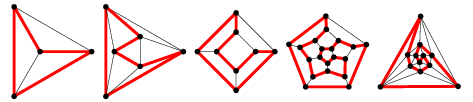
\includegraphics[width=\textwidth]{1.png}
\hfill \break
\hfill \break
As soon as the shell starts, it waits for the user to enter a command by displaying the command prompt \emph{osh$>$}. Once user enters a command, parent process will create a child process which in turn will parse the command. Once the command is parsed, the command will be passed on to the respective code snippet to execute the command accordingly. If the entered command is valid, then the child process will store that command in the history file and will pass on the control to the parent process. Parent process will continue to display command prompt and accepts commands as long as the user enters \emph{exit}. If the user enters \emph{exit}, then shell program ends. \\
\hfill \break
\pagebreak

\textbf{Design of each requirement specification} \\
\begin{enumerate}
    \item Execute basic commands:\\
    \hfill \break
We have used \emph{system} library function to execute commands which takes \emph{list} (array in perl) as an argument and returns 0 if it is successful and -1 if it fails. In the given \emph{list} array, first element should be the command and rest of the elements can be arguments of that command. \\
\hfill \break
 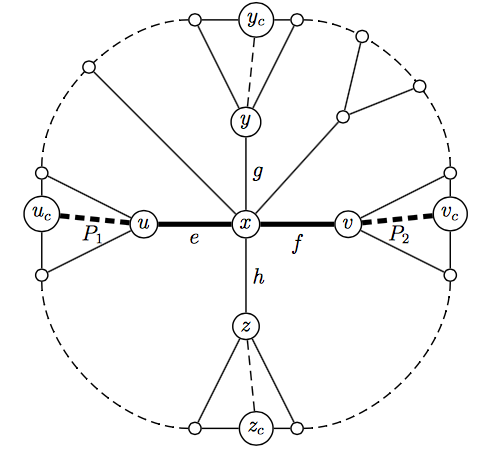
\includegraphics[scale=.8]{2.png}\\
 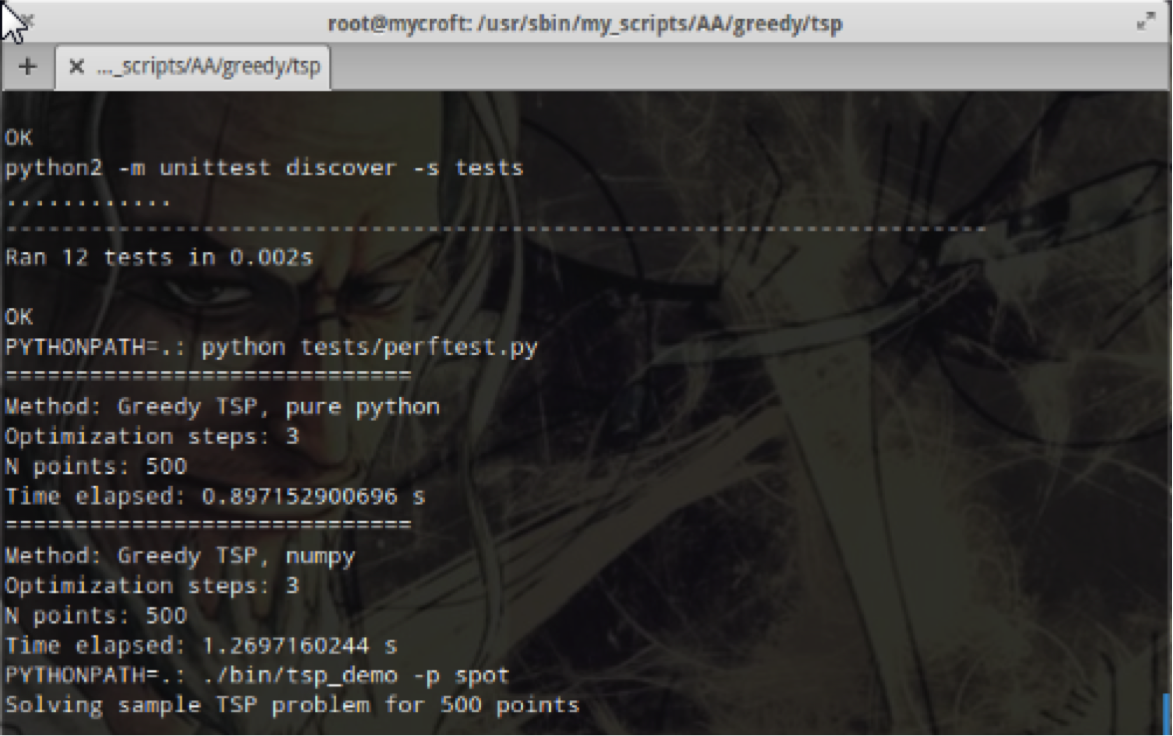
\includegraphics[scale=.8]{4.png}\\
\hfill \break
Above code prints the prompt and reads command from the user. It will loop until some valid command(text) is entered which means to ignore \emph{return} at command line. The last but one line tokenizes the command by using space as delimiter and stores command along with it's arguments in a list (array). In the end, \emph{system} exectes the entered command.
\hfill \break
    \item Commands in child process:\\
\hfill \break
\emph{fork()} is used to create child process and the entire processing happens in the child process only.\\
\hfill \break
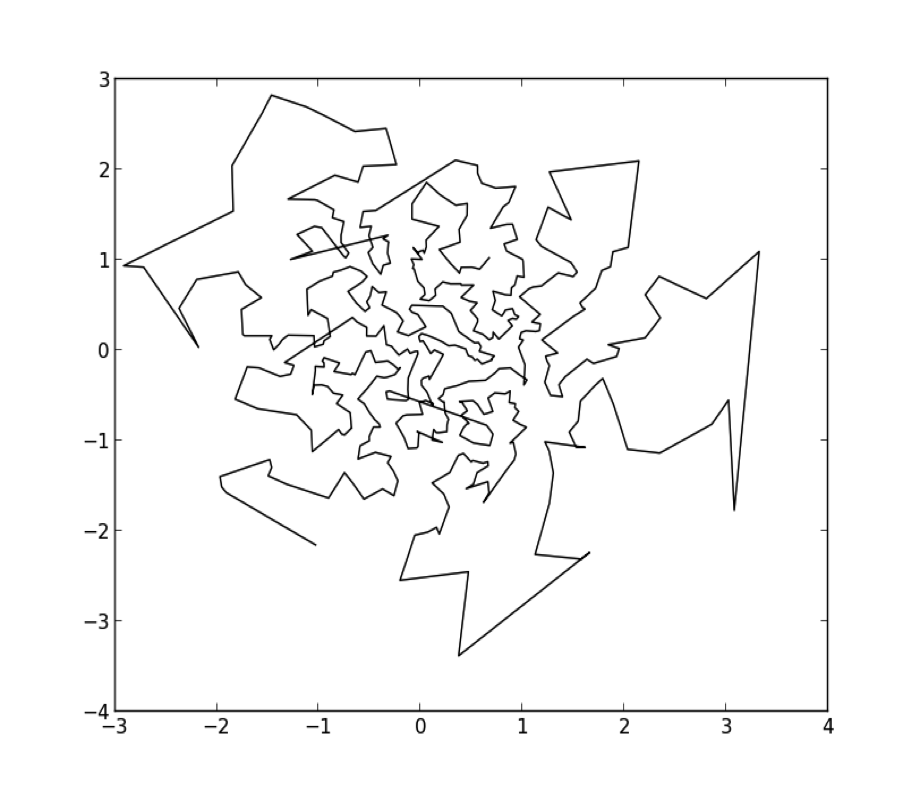
\includegraphics[scale=.8]{5.png}\\
\hfill \break
Above code snippet creates child process and check it's validity. Child process execution starts from the last line.
\hfill \break
\hfill \break
\hfill \break
    \item Background processing:\\
\hfill \break
In case of \emph{system} library function, fork is done first and parent process waits for the child process to exit. But, \emph{exec} library function on the other hand executes system command and never returns. So, if a user enters a command with an \emph{\&} in the end, we have used \emph{exec} library function as shown in the following code snippet.\\
\hfill \break
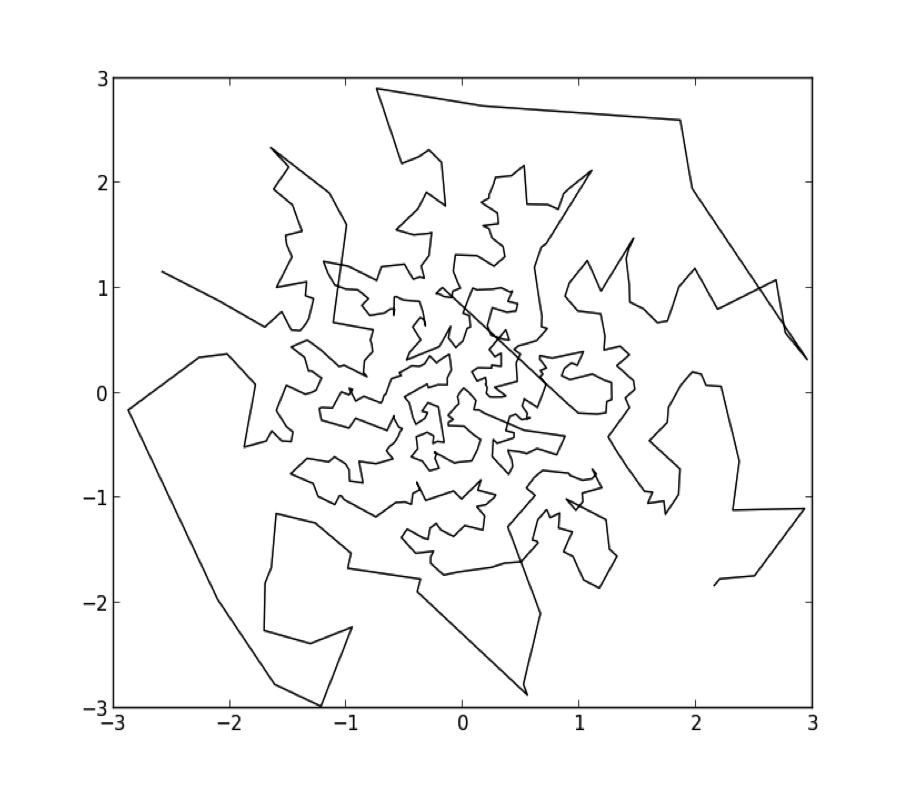
\includegraphics[scale=.8]{6.png}\\
\hfill \break
By using \emph{exec} function, parent process will not wait for the child process and will run concurrently with the child. Above code checks if the command ends with an \emph{\&} and executes using \emph{exec}.
\hfill \break
    \item \emph{history} festure:\\
\hfill \break
We have implemented \emph{history} feature by storing all the commands in a hidden text file in the current directory and maintaining two file pointers simultaneously to read and write to that file. One file pointer appends(writes) the commands executed at the end of the file and other pointer reads the contents of the file from bottom to top and stores the read commands in an array, which in turn can be displayed when user enters \emph{history} command.\\
\hfill \break
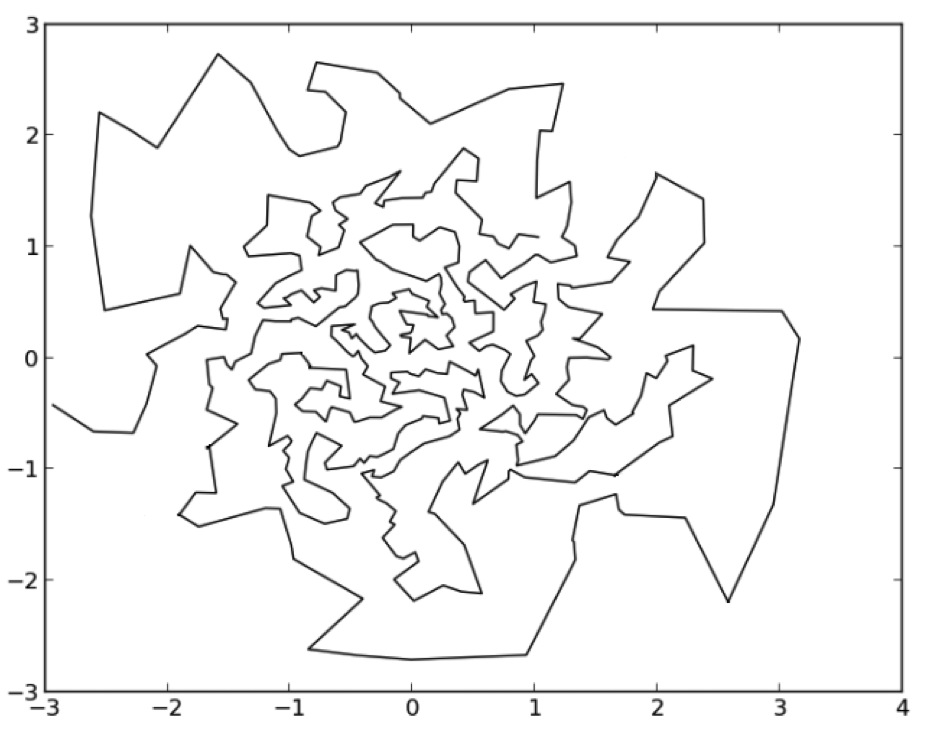
\includegraphics[scale=.8]{8.png}

In the above code, file pointer reads the history file from bottom to the top using the library function \emph{ReadBackwrds} and stores all the commands in an array.

    \item 10 most recent commands:\\
\hfill \break
\includegraphics[scale=.8]{9.png}\\
\hfill \break
Above code snippet displays the 10 most recent commands from the history. If there are less than 10 commands, it prints accordingly and stores itself( \emph{history} ) into the history.\\

    \item \emph{!!} -$>$ executes most recent command:\\
As we have already read the history file, we just need to execute the command available at index \emph{0} in the array of history commands to execute most recent one.\\
\hfill \break
\hfill \break
\hfill \break
\hfill \break
\hfill \break
\hfill \break
\hfill \break

\includegraphics[scale=.8]{10.png}\\

    \item \emph{!N} -$>$ execute N\textsuperscript{th} command:\\
\hfill \break
\includegraphics[scale=.8]{11.png}\\
\hfill \break
Above image contains a segment of code that handles single digit N value after ! and we have developed it to support 5 digit N value.\\
\hfill \break
\hfill \break
\hfill \break
\hfill \break



\end{enumerate}



\section{Issues and Challenges}
We have started developing the project using \emph{C} programming language and we had tough time handling string in C. It was also very challenging to maintain history. After developing half of the project, we have started developing it in both \emph{C} and as well as \emph{Perl}. We have completed both the versions successfully. We are submitting \emph{Perl} code as we were able to implement all the requirements and also have resolved most bugs that we came accross.

\section{Division of work}
Initially we three of us started working on different features individually. After completing one cycle of development, we segregated the work such that Prudhvi handled parser implementation, Madhulika worked in designing the workflow \& preparing the initial documentation part and I worked on history feature, other features and final documentation. We have also prepared a presentation to present it during demo, which can be found \href{http://prezi.com/io76sy9tsvnq/}{here}.\\

\section{Bibliography}

\textbf{[Abraham Silberschatz, Peter Baer Galvin and Greg Gagne 2013]} Abraham Silberschatz, Peter Baer Galvin and Greg Gagne, \emph{"Operating System Concepts"}, Wiley 2013.\\


\section{Final code}
Attached along with this document.

\end{document}